\documentclass[12pt, a4paper]{report}
\usepackage{graphicx, array, amsthm, amssymb, amsmath, algorithm, algpseudocode, float, xcolor, thmtools, thmbox}
\usepackage[english]{babel}

\makeatletter
\renewcommand\thmbox@headstyle[2]{\bfseries #1}
\makeatother
\newtheorem[style=M,bodystyle=\normalfont]{operation}{Operation}
\newtheorem[style=M,bodystyle=\normalfont]{theorem}{Theorem}
\newtheorem[style=M,bodystyle=\normalfont]{corollary}{Corollary}
\newtheorem[style=M,bodystyle=\normalfont]{lemma}{Lemma}
\newtheorem[style=M,bodystyle=\normalfont]{definition}{Definition}


\title{Formal Languages And Compilers \\ \textit{Theory}}
\author{Christian Rossi}
\date{Academic Year 2023-2024}

\begin{document}

\maketitle

\newpage

\begin{abstract}
    The lectures are about those topics: 
    \begin{itemize}
        \item Definition of language, theory of formal languages, language operations, regular expressions, regular languages, finite deterministic and non-deterministic automata, 
            BMC and Berry-Sethi algorithms, properties of the families of regular languages, nested lists and regular languages.
        \item Context-free grammars, context-free languages, syntax trees, grammar ambiguity, grammars of regular languages, properties of the families of context-free languages, 
            main syntactic structures and limitations of the context-free languages.
        \item Analysis and recognition (parsing) of phrases, parsing algorithms and automata, push down automata, deterministic languages, bottom-up and recursive top-down syntactic 
            analysis, complexity of recognition.
        \item Syntax-driven translation, direct and inverse translation, syntactic translation schemata, transducer automata, and syntactic analysis and translation. Definition of 
            semantics and semantic properties. Static flow analysis of programs. Semantic translation driven by syntax, semantic functions and attribute grammars, one-pass and 
            multiple-pass computation of the attributes.
    \end{itemize}
    The laboratory sessions are about those topics: 
    \begin{itemize}
        \item Modellization of the lexicon and the syntax of a simple programming language (C-like).
        \item Design of a compiler for translation into an intermediate executable machine language (for a register-based processor).
        \item Use of the automated programming tools Flex and Bison for the construction of syntax-driven lexical and syntactic analyzers and translators.
    \end{itemize}
\end{abstract}

\newpage

\tableofcontents

\newpage

\chapter{Regular Languages}
    \subsection{Formal language theory}
    A \emph{formal language} consists of words whose letters are taken from an alphabet and are well-formed according to a specific set of rules.
    \begin{definition}
        An \emph{alphabet} is a finite set of elements called terminal symbols or \emph{characters}. 
        The \emph{cardinality} of an alphabet \[\Sigma =\{ a_1,a_2,\dots, a_k \}\] is the number of characters that it contains: $\left\lvert \Sigma \right\rvert = k$. 
        A \emph{string} or word is a sequence of characters. 
    \end{definition}
    \begin{example}
        The alphabet $\Sigma =\{ a,b \}$ has a cardinality of two. Some possible languages derived from this alphabet can be:
        \begin{itemize}
            \item $L_1=\{aa,aaa\}$
            \item $L_2=\{aba,aab\}$
            \item $L_3=\{ab,ba,aabb,abab,\dots,aaabbb,\dots\}$
        \end{itemize}
    \end{example}
    \begin{definition}
        Given a language, a string belonging to it is called a \emph{sentence} or \emph{phrase}. The \emph{cardinality} or size of a language is the number of sentence it contains.
        If the cardinality is finite, the language is called \emph{vocabulary}. 
    \end{definition}
    \begin{example}
        Given the language (that is a vocabulary) $L_2=\{ bc,bbc \}$ we have that its cardinality is equal to two. 
    \end{example}
    \begin{definition}
        The number of repetitions of a certain letter in a word is called \emph{number of occurrences}. The \emph{length} of a string is the number of its elements. 
        Two strings are \emph{equal} if and only if: 
        \begin{itemize}
            \item They have the same length.
            \item Their elements, from left to right, coincide. 
        \end{itemize}
    \end{definition}
    \begin{example}
        The number of occurrences of $a$ and $c$ in $aab$ is indicated with:
        \[{\left\lvert aab \right\rvert}_a = 2\]
        \[{\left\lvert aab \right\rvert}_c = 0\]
        The length of the string $aab$ is equal to: 
        \[\left\lvert aab \right\rvert = 3\]
    \end{example}
    
    \subsection{Operations on strings}
    \begin{operation}[Concatenation]
        Given two strings $x=a_1a_2\dots a_h$ and $y=b_1b_2\dots b_k$ the \emph{concatenation} is defined as:
        \[x \cdot y = a_1a_2\dots a_h b_1b_2\dots b_k\]
    \end{operation}
    Concatenation is non-commutative and associative ($x(yz)=(xy)z$). The length of the result is the sum of the length of the concatenated strings
    ($\left\lvert xy \right\rvert = \left\lvert x \right\rvert + \left\lvert y \right\rvert$). 
    \begin{operation}[Empty string]
        The \emph{empty string} $\varepsilon$ is the neutral element for concatenation that satisfies the identity:
        \[x\varepsilon=\varepsilon x=x\]
    \end{operation}
    It is important to note that $\left\lvert \varepsilon \right\rvert = 0$ and that the set that contains this operator is not the empty set. 
    \begin{operation}[Substring]
        Let string $x=xyv$ be written as the concatenation of three, possibly empty, strings $x,y$ and $v$. Then, strings $x,y$ and $v$ are \emph{substrings} of $x$. 
    \end{operation}
    Moreover, string $u$ is a prefix of $x$ and $v$ is a suffix of $x$. A non-empty substring is called proper if it does not coincide with string $x$. 
    \begin{operation}[Reflection]
        The \emph{reflection} of a string $x=a_1a_2\dots a_h$ is:
            \[x^R=a_ha_{h-1}\dots a_1\]
    \end{operation}
    The following identities are immediate: 
    \[(x^R)^R=x \:\:\:\:\:\: (xy)^R=y^Rx^R \:\:\:\:\:\: \varepsilon^R=\varepsilon\]
    \begin{operation}[Repetition]
        The \emph{repetition} is the $m$-th power $x^m$ of a string $x$ is the concatenation of $x$ with himself $m-1$ times. The formal definition o the following: 
        \[x^m=x^{m-1}x \:\: for m \geq 1 \:\:\:\:\:\: x^0=\varepsilon\]
    \end{operation}
    Repetition and reflection take precedence over concatenation. 

    \subsection{Operations on languages}
    Operations are typically defined on a language by extending the string operation to all its phrases. 
    \begin{operation}[Reflection]
        The \emph{reflection} $L^R$ of a language $L$ is the finite set of strings that are the reflection of a sentence of $L$: 
        \[L^R = \{ x | \exists y \left( y \in L \land x=y^R \right)\}\]
    \end{operation}
    \begin{operation}[Prefix]
        The set of \emph{prefixes} of a language $L$ is defined as: 
        \[Prefixes(L)=\{y | y \neq \varepsilon \land \exists x \exists z \left( x \in L \land x=yx \land z \neq \varepsilon \right)\}\]
    \end{operation}
    A language is prefix-free if none of the proper prefixes of its sentences is in the language. 
    \begin{operation}[Concatenation]
        Given languages $L^{'}$ and $L^{''}$ we have that \emph{concatenation} is defined as: 
            \[L^{'}L^{''}=\{ xy | x \in L^{'} \land y \in L^{''} \}\]
    \end{operation}
    \begin{operation}[Repetition]
        The \emph{repetition} is redefined as: 
        \[L^m=L^{m-1}L \:for \: m \geq 1 \:\:\:\:\:\: L^0=\{ \varepsilon \}\]
    \end{operation}
    The identity now became: 
    \[\varnothing ^0 = \{ \varepsilon \} \:\:\:\:\:\: L.\varnothing=\varnothing .L=\varnothing \:\:\:\:\:\: L.\{\varepsilon\}=\{\varepsilon\} .L=L\]
    The power operator allows one to define concisely the language of strings whose length is not greater than a given integer $K$. 
    \begin{operation}[Set operations]
        Since a language is a set, the classical set operation of union ($\cup$), intersection ($\cap$), difference ($ \setminus $), inclusion ($ \subseteq $), strict inclusion 
        ($ \subset $), and equality ($=$). 
    \end{operation}
    \begin{operation}[Universal language]
        The \emph{universal language} is defined as the set of all the strings, over an alphabet $\Sigma$, of any length including zero: 
        \[L_{universal}=\Sigma ^0 \cup \Sigma ^1 \cup \Sigma ^2 \cup \dots \]
    \end{operation}
    \begin{operation}[Complement]
        The \emph{complement} of a language $L$ over an alphabet $\Sigma$, denoted by $\lnot L$, is the set difference: 
            \[ \lnot L = L_{universal} - L\]
    \end{operation}
    That is, the set of the strings over the alphabet $\Sigma$ that are not in $L$. Note that: 
    \[L_{universal} = \lnot \varnothing\]
    The complement of a finite language is always infinite. The complement of an infinite one is not necessarily finite.   

    Given a set A and a relation $R \subseteq A \times A$, $(a_1, a_2) \in R$ is also denoted as $a_1Ra_2$. $R^{*}$ is a relation defined by:
    \begin{itemize}
        \item $xR^{*}x \:\: \forall x \in A$ (reflexive property). 
        \item $x_1Rx_2 \land x_2Rx_3 \land \dots x_{n-1}Rx_n \implies x_1R^{*}x_n$ (transitive property). 
    \end{itemize}
    \begin{example}
        Given $R = \{(a, b), (b, c)\}$, the transitive closure will be: 
        \[R^{*} = \{(a, a), (b, b), (c, c), (a, b), (b, c), (a, c) \}\]
    \end{example}
    Given a set A and a relation $R \subseteq A \times A$, $(a_1, a_2) \in R$ is also denoted as $a_1Ra_2$. $R^{+}$ is a relation defined by: 
    $x_1Rx_2 \land x_2Rx_3 \land \dots x_{n-1}Rx_n \implies x_1R^{*}x_n$ (transitive property). 

    \begin{example}
        Given $R = \{(a, b), (b, c)\}$, the transitive closure will be: 
        \[R^{+} = \{ (a, b), (b, c), (a, c)\}\]
    \end{example}
    \begin{operation}[Star operator]
        The \emph{star operator} (also called Kleene star) is the reflexive transitive closure under the concatenation operation. It is defined as the union of all the powers of the 
        base language: 
        \[L^{*}=\bigcup_{h=0\dots\infty}L^h=L^0 \cup L^1 \cup L^2 \cup \dots = \varepsilon \cup L^1 \cup L^2 \cup \dots\]
    \end{operation}
    \begin{example}
        Given the language $L=\{ab,ba\}$ we have that the star operation gives the following language: 
        \[L^{*}=\{\varepsilon, ab, ba, abab, abba, baab, baba, \dots\}\]
        It is possible to see that $L$ is finite and $L^{*}$ is infinite. 
    \end{example}
    Every string of the star language $L^{*}$ can be chopped into substrings in $L$. The star language $L^{*}$ can be equal to the base language $L$. If we take $\Sigma$ as the base 
    language, then $\Sigma^{*}$ contains all the strings built on that alphabet (it is the universal language of alphabet $\Sigma$). We often say that $L$ is a language on alphabet
    $\Sigma$ by writing $L \subseteq \Sigma$. 
    \begin{table}[H]
        \centering
        \begin{tabular}{cc}
        \hline
        \textbf{Property}                                      & \textbf{Meaning}            \\ \hline
        $L \subseteq L^{*}$                                    & Monotonicity                \\
        if $x \in L^{*} \land y \in L^{*}$ then $xy \in L^{*}$ & Closure by concatenation    \\
        $(L^{*})^{*}=L^{*}$                                    & Idempotence                 \\
        $(L^{*})^R=(L^R)^{*}$                                  & Commutativity with reversal \\ \hline
        \end{tabular}
    \end{table}
    Furthermore, if $L^{*}$ is finite we have $\varnothing^{*}=\{\varepsilon\}$ and that $\{\varepsilon\}^{*}=\{\varepsilon\}$. 
    \begin{operation}[Cross operator]
        The \emph{cross operator} is the transitive closure under the concatenation operation. It is defined as the union of all the powers of the 
        base language except the first power $L^0$: 
        \[L^{+}=\bigcup_{h=1\dots\infty}L^h=L^1 \cup L^2 \cup \dots\]
    \end{operation}
    \begin{example}
        Given the language $L=\{ab,ba\}$ we have that the star operation gives the following language: 
        \[L^{*}=\{ab, ba, abab, abba, baab, baba, \dots\}\]
    \end{example}
    \begin{operation}[Language quotient]
        The \emph{quotient operator} shortens the phrases of $L_1$ by cutting off a suffix that belongs to $L_2$:
        \[L=L_1/L_2=\{y|\exists x \in L_1 \exists y \in L_2 (x=yz)\}\]
    \end{operation}
    \begin{example}
        Given the languages $L_1=\{a^{2n}b^{2n}|n>0\}$ and $L_2=\{b^{2n+1}|n \geq 0\}$ the quotient language is: 
        \[L=L_1/L_2=\{aab,aaaab,aaaabbb\}\]
    \end{example}

    \subsection{Regular expressions and languages}
    The family of regular languages is our simplest formal language family. It can be defined in three ways: algebraically, by means of generative grammars, and by means of 
    recognizer automata. 
    \begin{definition}
        A \emph{regular expression} is a string $r$ containing the terminal characters of the alphabet $\Sigma$ and the following meta-symbols: union ($\cup$), concatenation ($.$), 
        star ($^{*}$), empty string ($\varepsilon$), and parenthesis in accordance with the following rules:
        \begin{table}[H]
            \centering
            \begin{tabular}{|cc|}
            \hline
            $r=\varepsilon$ & Empty string                 \\
            $r=a$           & Unitary language             \\
            $r=s \cup t$    & Union of expressions         \\
            $r=(st)$        & Concatenation of expressions \\
            $r=s^{*}$       & Iteration of an expression   \\ \hline
            \end{tabular}
        \end{table}
        where the symbols $s$ and $t$ are regular sub-expression. 
    \end{definition}
    For expressivity, the metasymbol cross is allowed. The operators precedence is: star, concatenation, and union. 
    \begin{definition}
        A \emph{regular language} is a language denoted by a regular expression. 

        The \emph{family of regular languages} (REG) is the collection of all regular languages. 

        The \emph{family of finite languages} (FIN) is the collection of all languages having a finite cardinality
    \end{definition}
    We have that every finite language is regular because it is the union of a finite number of strings each one being the concatenation of a finite 
    number of alphabet symbols. The family of regular languages also includes languages having infinite cardinality (hence $FIN \subset REG$)
    
    The union and repetition operators correspond to possible choices. One obtains a sub-expression by making a choice that identifies a sub-language. Given a regular expression 
    one can derive another one by replacing any outermost sub-expression with another that is a choice of it. 
    \begin{definition}
        We say that a regular expression $e^{'}$ \emph{derives} a regular expression $e^{''}$, written $e^{'} \implies e^{''}$, if the two regular expressions can be factorized as 
        \[e^{'}=\alpha \beta \gamma \:\:\:\:\:\: e^{''}=\alpha \delta \gamma\]
        where $\delta$ is a choice of $\beta$.
    \end{definition}
    The derivation relation can be applied repeatedly, yielding relation $\implies^{n}$ ($n$ steps), $\implies^{*}$ ($n \geq 0$ steps), and $\implies^{+}$ ($n > 0$ steps). 
    \begin{definition}
        Two regular expressions are \emph{equivalent} if they define the same language. 

        A regular expression is \emph{ambiguous} if the language of the numbered version $f^{'}$ includes two distinct strings $x$ and $y$ that coincide when numbers are erased. 
    \end{definition}

    \newpage 

    \chapter{Grammars}
        \section{Context-free generative grammars}
        Regular expressions are very practical for describing lists but fall short of the capacity needed to define other frequently occurring constructs. 
        For defining other useful languages, regular or not, we move to the formal model of generative grammars.  A generative grammar or syntax is a set of multiple 
        rules that can be repeatedly applied in order to generate all and only the valid strings. 
        \begin{definition}
            A \emph{context-free grammar} $G$ is defined by four entities: 
            \begin{enumerate}
                \item $V$ non-terminal alphabet, is the set of non-terminal symbols.
                \item $\Sigma$ terminal alphabet, is the set of the symbols of which phrases or sentences are made.
                \item $P$ is the set of rules or productions.
                \item $S \in V$ is the specific non-terminal, called the axiom ($S$), from which derivations start. 
            \end{enumerate}
        \end{definition}
        A rule of set $P$ is an order pair $X \rightarrow \alpha$, with $X \in V$ and $\alpha \in (V \cup \Sigma)^{*}$. Two or more rules: 
        \[X \rightarrow \alpha_1 \:\:\:\: X \rightarrow \alpha_2 \:\:\:\: \dots \:\:\:\: X \rightarrow \alpha_n\]
        with the same left part $X$ can be concisely groped in:
        \[X \rightarrow \alpha_1 | \alpha_2 | \dots | \alpha_n\]
        We say that the strings $\alpha_1,\alpha_2,\dots,\alpha_n$ are the alternative of $X$. 
    
        \subsection{Conventional grammar representation}
        In professional practice, different styles are used to represent terminals and non-terminals. We usually adopt these conventions: 
        \begin{itemize}
            \item Lowercase Latin letters $\{a,b,\dots\}$ for terminal characters. 
            \item Uppercase Latin letters $\{A,B,\dots\}$ for non-terminal symbols. 
            \item Lowercase Latin letters $\{r,s,\dots,z\}$ for strings over the alphabet $\Sigma$. 
            \item Lowercase Greek letters $\{r,s,\dots,z\}$ for both terminals and non. 
            \item $\sigma$ only for non-terminals. 
        \end{itemize}
        The classification of grammar rule forms is the following. 
        \begin{figure}[H]
            \centering
            \includegraphics[width=1\linewidth]{images/grammars.png}
        \end{figure}
    
        \subsection{Derivation and Language Generation}
        We reconsider and formalize the notion of string derivation. Let $\beta=\delta A \eta$ be a string containing a non-terminal, where $\delta$ and $\eta$ are any, 
        possibly empty strings. Let $A \rightarrow \alpha$ be a rule of $G$ and let $\gamma=\delta\alpha\eta$ be the string obtained replacing in $\beta$ non-terminal $A$with 
        the right part $\alpha$. The relation between such two strings is called derivation. We say that $\beta$ derives $\gamma$ for grammar $G$, written:
        \[\beta \implies \gamma\]
        $A\rightarrow \alpha$ is applied in such derivation and string $\alpha$ reduced to non-terminal $A$. The possible closures are: power ($\implies^n$), 
        reflexive ($\implies^{*}$), and transitive ($\implies^{+}$). 
        \begin{definition}
            If $A \implies^{*} \alpha$ we have that $\alpha \in (V \cup \Sigma)$ is called \emph{string form} generated by $G$. 
    
            If $S \implies^{*} \alpha$ we have that $\alpha$ is called \emph{sentential} or phrase form.
    
            If $A \implies^{*} s$ we have that $s \in \Sigma^{*}$ is called \emph{phrase} or sentence. 
    
            Language is \emph{context-free} if a context-free grammar exists that generates it. 
            
            Two grammars $G$ and $G^{'}$ are \emph{equivalent} if they generate the same language. 
        \end{definition}
    
        \subsection{Erroneous grammars and useless rules}
        When writing a grammar attention should be paid that all non-terminals are defined and that each one effectively contributes to the production of some sentence. 
        In fact, some rules may turn out to be unproductive. 
        \begin{definition}
            A grammar $G$ is called \emph{clean} (or reduced) under the following conditions:
            \begin{enumerate}
                \item Every non-terminal $A$ is reachable from the axiom.
                \item Every non-terminal $A$ is well-defined.
            \end{enumerate}
        \end{definition}
        It is often straightforward to check by inspection whether a grammar is clean. The following algorithm formalizes the checks. The algorithm operates in two phases, 
        first pinpointing the undefined non-terminals, then the unreachable ones. Lastly the rules containing non-terminals of either type can be canceled. The phases are: 
        \begin{enumerate}
            \item Compute the set $DEF\subseteq V$ of well-defined non-terminals. The set $DEF$ is initialized with the non-terminals of terminal rules, those having a 
                terminal string as right part:
                \[DEF:=\{A|( A \rightarrow u ) \in P,with u \in \Sigma^{*}\}\]
                Then the next transformation is applied until convergence is reached:
                \[DEF:=DEF \cup B|( B \rightarrow D_1D_2\dots D_n)\in P\]
                where every $D_i$ is a terminal or a non-terminal symbol present in $DEF$. At each iteration two outcomes are possible:
                \begin{itemize}
                    \item A new non non-terminal is found having as right part a string of symbols that are well-defined non-terminals or terminals. 
                    \item The termination condition is reached
                \end{itemize}
                The non-terminals belonging to the complement set $V-DEF$ are undefined and should be eliminated.
            \item A non-terminal is reachable from the axiom, if, and only if, there exists a path in the following graph, which represents a relation between non-terminals,
                called product:
                \[A \rightarrow^{produce} B\]
                saying that $A$ produces $B$ if, and only if, there exists a rule $A \rightarrow \alpha B \beta$, where $A,B$ are non-terminals and $\alpha,\beta$ are any strings.
                Clearly $C$ is reachable from $S$ if, and only if, in this graph there exists an oriented path from $S$ to $C$. The unreachable non-terminals are the complement
                with respect to $V$. They should be eliminated because they do not contribute to the generation of any sentence.
        \end{enumerate}
        Quite often the following requirement is added to the above clearness conditions: $G$ should not permit circular deviations $A \implies^{+} A$. This is done to avoid 
        ambiguity. We observe that a grammar, although clean, may still contain redundant rules. 
    
        \subsection{Recursion and language infinity}
        An essential property of most technical languages is to be infinite. We study how this property follows from the form of grammar rules. In order to generate an 
        unbound number of strings, the grammar must be able to derive strings of unbound length. To this end, recursive rules are necessary, as next argued. An $n \geq 1$ 
        steps derivation $A \implies^{n}xAy$ is called recursive (immediately recursive if $n=1$); similarly non-terminal $A$ is called recursive. If $x$ is empty, the recursion 
        is termed left.
    
        Let $G$ be a grammar clean and avoid of circular deviations. The language $L ( G )$ is infinite if, and only if, $G$ has a recursive derivation.
    
        \subsection{Syntax trees and canonical derivations}
        \begin{definition}
            A \emph{tree} is an oriented and ordered graph not containing a circuit, such that every pair of nodes is connected by exactly one oriented path.
            
            An \emph{arc} $\langle N_1,N_2 \rangle$ define the $\langle \textnormal{father,son} \rangle$ relation, customarily visualized from top to bottom as in genealogical 
            trees. The sides of a node are ordered from left to right. 
    
            The \emph{degree} of a node is the number of its siblings. 
            
            A \emph{tree} contains one node without father, termed root.
    
            Consider an internal node $N$: the subtree with root $N$ is the tree having $N$ as root and containing all descendants of $N$. Nodes without sibling are termed leaves or \emph{terminal nodes}. 
        
            The sequence of all leaves, read from left to right, is the \emph{frontier} of the tree.
    
            A \emph{syntax tree} has as root the axiom and as frontier a sentence.
        \end{definition}
        A syntax tree of a sentence $x$ can also be encoded in a text, by enclosing each subtree between brackets. Brackets are subscribed with the non-terminal symbol. The representation can be simplified 
        by dropping the non-terminal labels, thus obtaining a skeleton tree. A further simplification of the skeleton tree consists in shortening non bifurcating paths, resulting in the condensed skeleton tree. 
    
    
        \subsection{Left and right derivations}
        We can have right (expands at each step the rightmost non-terminal) and left derivation (expands at each step the leftmost non-terminal). 
        However, for a fixed syntax tree of a sentence, there exist a unique right derivation, and a unique left derivation matching that tree. Right and left derivation are useful to define parsing algorithms. 
    
        \subsection{Parenthesis languages}
        Many  artificial  languages  include  parenthesized  or  nested  structures,  made  by matching pairs of opening/closing marks. Any such occurrence may contain other matching pairs.
        The marks are abstract elements that have different concrete representations indistinct settings.
        \begin{definition}
            When a marked construct may contain another construct of the same kind, it is called \emph{self-nested}.
        \end{definition}
        Self-nesting is potentially unbounded in artificial languages, whereas in natural languages its use is moderate, because it causes difficulty of comprehension by breaking the flow of discourse. 
        Abstracting from concrete representation and content, this paradigm is known as a Dyck language. The terminal alphabet contains one or more pairs of opening/closing marks. 
        Dyck sentences are characterized by the following cancelation rule that checks parentheses are well nested: given a string, repeatedly substitute the empty string for a pair of adjacent matching parentheses:
        \[[\:]\implies\varepsilon \:\:\:\:\:\: (\:)\implies\varepsilon\]
        Thus obtaining another string. Repeat until the transformation no longer applies; the original string is correct if, and only if, the last string is empty.
        \begin{definition}
            Let $G=(V,\Sigma,P,S)$ be a grammar with an alphabet $\Sigma$ not containing parentheses. The \emph{parenthesized grammar} $G_p$ has alphabet $\Sigma \cup \{'(',')'\}$ and rules:
            \[A \rightarrow (\alpha) \textnormal{ where } A \rightarrow (\alpha) \textnormal{ is a rule of } G\]
            The grammar is distinctly parenthesized if every rule has form:
            \[A \rightarrow (_A \alpha)_A \:\:\:\:\:\: B \rightarrow (_B \alpha)_B\]
            where $(_A$ and $)_A$ are parentheses subscripted with the non-terminal name.
        \end{definition}
        Clearly each sentence produced by such grammars exhibits parenthesized structure. A notable effect of the presence of parentheses is to allow a simpler checking of string correctness. 
    
        \subsection{Regular composition of context-free languages}
        If the basic operations of regular languages, union, concatenation, and star, are applied to context-free languages, the result remains a member of the CF family. Let $G_1=(\Sigma_1,V_1,P_1,S_1)$
        and $G_2=(\Sigma_2,V_2,P_2,S_2)$ be the grammars defining languages $L_1$ and $L_2$. We need the not restrictive hypothesis that non-terminal sets are disjoint. Moreover, we stipulate that symbol $S$, 
        to be used as axiom of the grammar under construction, is not used by either grammar, $S \notin (V_1 \cup V_2)$.
        \begin{operation}[Union]
            The union $L_1 \cup L_2$ is defined by the grammar containing the rules of both grammars, plus the initial rules $S\rightarrow S_1|S_2$. In formulas, the grammar is: 
            \[G=\left(\Sigma_1 \cup \Sigma_2,\{S\} \cup V_1 \cup V_2,\{S\rightarrow S_1|S_2\} \cup P_1 \cup P_2,S\right)\]
        \end{operation}
        \begin{operation}[Concatenation]
            The concatenation $L_1L_2$ is defined by the grammar containing the rules of both grammars, plus the initial rule $S\rightarrow S_1S_2$. The grammar is: 
            \[G=\left(\Sigma_1 \cup \Sigma_2,\{S\} \cup V_1 \cup V_2,\{S\rightarrow S_1S_2\} \cup P_1 \cup P_2,S\right)\] 
        \end{operation}
        \begin{operation}[Star]
            The grammar $G$ of the starred language $(L1)^{*}$ includes the rules of $G_1$ and rules $S \rightarrow SS_1|\varepsilon$.
        \end{operation}
        \begin{operation}[Cross]
            From the identity $L^{+}=L.L^{*}$, the grammar of the cross language could be written applying the concatenation construction to $L$ and $L^{*}$, but it is better to produce the grammar directly. 
            The grammar $G$ of language $(L1)^{+}$ contains the rules of $G_1$ and rules $S \rightarrow SS_1|S1$. 
        \end{operation}
        The family CF of context-free languages is closed by union, concatenation, star, and cross. Examining the effect of string reversal on the sentences of a CF language, one immediately sees the family 
        is closed with respect to reversal (the same as family REG). Given a grammar, the rules generating the mirror language are obtained reversing every right part of a rule.

        \subsection{Ambiguity}
        The common linguistic phenomenon of ambiguity in natural language shows up when a sentence has two or more meanings. Ambiguity is of two kinds, semantic or syntactic.
        \begin{definition}
            A sentence $x$ defined by grammar $G$ is \emph{syntactically ambiguous}, if it is generated with two different syntax trees. Then the grammar too is called ambiguous.

            The \emph{degree of ambiguity} of a sentence $x$ of  language $L(G)$ is the number of distinct syntax trees deriving the sentence. For a grammar the degree of ambiguity is the maximum degree of 
            any ambiguous sentence.
        \end{definition}
        The ambiguity can be: 
        \begin{itemize}
            \item From bilateral recursion
        \end{itemize}


        PAG 47 A 79

        \subsection{Grammar transformations and normal forms}
        The grammars can be transformed in the following ways: 
        \begin{itemize}
            \item 
        \end{itemize}

\newpage

\chapter{Finite state automata}
    \section{Recognition algorithms and automata}
    To check if a string is valid for a specified language, we need a recognition algorithm, a type of algorithm producing a yes/no answer, commonly referred to in 
    computational complexity studies as a decision algorithm. For the string membership problem, the input domain is a set of strings of alphabet $\Sigma$. The 
    application of a recognition algorithm $\alpha$ to a given string $x$ is denoted as $\alpha(x)$. We say string $x$ is recognized or accepted if $\alpha(x)=yes$, 
    otherwise it is rejected. The language recognized, $L(\alpha)$, is the set of accepted strings:
    \[L(\alpha)=\{x \in \Sigma^{*}|\alpha(x)=yes\}\]
    The algorithm is usually assumed to terminate for every input, so that the membership problem is decidable. However, it may happen that, for some string $x$,the 
    algorithm does not terminate. In such case we say that the membership problem for $L$ is semi-decidable, or also that $L$ is recursively enumerable. In practice, 
    we do not have to worry about such decidability issues because in language processing the only language families of concern are decidable. 
    \subsection{A general automaton}
    An automaton or abstract machine is an ideal computer featuring a very small set of simple instructions. In its more general form a recognizer it is composed by three 
    parts: input tape, control unit, and (auxiliary) memory. The control unit has a limited store, to be represented as a finite set of states;the auxiliary memory, on the 
    other hand, has unbounded capacity. The upper tape contains the given input or source string, which can be read but not changed. Each case of the tape contains a 
    terminal character; the cases to the left and right of the input contain two delimiters, the start of text mark $\vdash$ and the end of text mark or terminator $\dashv$.
    A peculiarity of automata is that the auxiliary memory is also a tape containing symbols of another alphabet. The automaton examines the source by performing a series
    of moves; the choice of a move depends on the current two symbols (input  and  memory) and on the current state. A move may have some of the following effects:
    \begin{itemize}
        \item Shift the input head left or right by one position. 
        \item Overwrite the current memory symbol with another one, and shift the memory head left or right by one position. 
        \item Change the state of the control unit.
    \end{itemize}
    \begin{definition}
        A machine is \emph{unidirectional} if the input head only moves from left to right. 
    \end{definition}
    At any time the future behavior of the machine depends on a three-tuple, called configuration: the suffix of the input string still to be read, the contents of the 
    memory tape and the position of the head. 
    \begin{definition}
        The \emph{initial configuration} has: the input head positioned on character $a_1$, the control unit in an initial state, and the memory containing a specific 
        symbol.
    \end{definition}
    Then the machine performs a computation. If for a configuration at most one move can be applied, the change of configuration is deterministic. A non-deterministic
    automaton is essentially a manner of representing an algorithm that in some situation may explore alternative paths. 
    \begin{definition}
        A configuration is \emph{final} if the control is in a state specified as final, and the input head is on the terminator. 
    \end{definition}
    The source string $x$ is accepted if the automaton, starting in the initial configuration with $x\dashv$ as input, performs a computation leading to a final configuration. 
    The language accepted or recognized by the machine is the set of accepted strings.

    Notice a computation terminates either when the machine has entered a final con-figuration or when in the current configuration no move can be applied. In the latter 
    case the source string is not accepted by that computation. 
    \begin{definition}
        Two automata accepting the same language are called \emph{equivalent}.
    \end{definition}

    \section{Introduction to finite automata}
    Conforming to the general scheme, a finite automaton comprises: the input tape with the source string $x \in \Sigma^{*}$, the control unit, and the reading head scanning 
    the string until its end, unless an error occurs before. Upon reading a character, the automaton updates the state  of the  control unit and advances the reading head. 
    Upon reading the last character, the automaton accepts $x$ if and only if the state is an accepting one.

    A well-known representation of an automaton is by a state-transition diagram or graph. This is a directed graph whose nodes are the states of the control unit. Each arc
    is labeled with a terminal and represents the change of state or transition caused by reading the terminal.

    An automaton may have several final states, but only one initial state. 

    \section{Deterministic finite automata}
    \begin{definition}
        A \emph{finite deterministic automaton M} comprises five items:
        \begin{enumerate}
            \item $Q$, the state set (finite and not empty). 
            \item $\Sigma$, the input or terminal alphabet
            \item $\delta:(Q \times \Sigma) \rightarrow Q$, the transition function.
            \item $q_0 \in Q$, the initial state. 
            \item $F\subseteq Q$, the set of final states.
        \end{enumerate}
    \end{definition}
    Function $\delta$ specifies the moves: the meaning of $\delta(q,a)=r$ is that machine $M$ in the current state $q$ reads $a$ and moves to next state $r$. 
    If $\delta(q,a)$ is undefined, the automaton stops, and we can assume it enters the error state. 

    A special case is the empty string, for which we assume no change of state: 
    \[\forall q \in Q:\delta(q,\varepsilon)=q\]
    \begin{definition}
        The languages accepted by such automata are called \emph{finite-state recognizable}.
        
        Two automata are \emph{equivalent} if they accept the same language.
    \end{definition}
    Observing that for each input character the automaton executes one step, the total number of steps is exactly equal to the length of the input string. Therefore, such
    machines are very efficient as they can recognize strings in real time by a single left-to-right scan.

    \subsection{Error state and total automata}
    If the move is not defined in state $q$ when reading character $a$, we say that the automaton falls into the error state $q_{err}$. The error state is such that for 
    any character the automaton remains in it, thus justifying its other name of sink or trap state. Obviously the error state is not final. The state-transition function 
    can be made total by adding the error state and the transitions from/to it. 

    Clearly any computation reaching the error state gets trapped in it and cannot reach a final state. As a consequence, the total automaton accepts the same language as 
    the original one. It is customary to leave the error state implicit, neither drawing a node nor specifying the transitions for it.

    \subsection{Clean automata}
    An automaton may contain useless parts not contributing to any accepting computation, which are best eliminated.
    \begin{definition}
        A state $q$ is \emph{reachable} from state $p$ if a computation exists going from $p$ to $q$.

        A state is \emph{accessible} if it can be reached from the initial state. 

        A state is \emph{post-accessible} if a final state can be reached from it. 

        A state is called \emph{useful} if it is accessible and post-accessible. 

        An automaton is \emph{clean} if every state is useful.
    \end{definition}
    For every finite automaton there exists an equivalent clean automaton.

    \subsection{Minimal automata}
    For every finite-state language, the deterministic finite recognizer minimal with respect to the number of states is unique.
    \begin{definition}
        The states $p$ and $q$ are \emph{indistinguishable} if, and only if, for every string $x \in \Sigma^{*}$, either both states $\delta(p,x)$ and $\delta(q,x)$ are 
        final, or neither one is. 
        
        The complementary relation is termed \emph{distinguishability}.
    \end{definition}
    Two states $p$ and $q$ are indistinguishable if, starting from them and scanning the same arbitrarily chosen input string $x$, it never happens that a computation 
    reaches a final state and the other does not. Notice that: 
    \begin{enumerate}
        \item The sink state $q_{err}$ is distinguishable from every state $p$, since for any state there exists a string $x$ such that $\delta(p,x) \in F$, while for 
            every string $x$ it is $\delta(q_{err},x)=q_{err}$. 
        \item $p$ and $q$ are distinguishable if $p$ is final and $q$ is not, because $\delta(p,\varepsilon)\in F$ and $\delta(q,\varepsilon) \notin F$. 
        \item $p$ and $q$ are distinguishable if, for some character $a$, the next states $\delta(p,a)$ and $\delta(q,a)$ are distinguishable.
    \end{enumerate}
    In particular, $p$ is distinguishable from $q$ if the set of labels attached to the outgoing arrows from $p$ and the similar set from $q$ are different. 

    Indistinguishability as a relation is symmetric, reflexive, and transitive. 

    \subsection{Construction of minimal automaton}
    The minimal automaton $M^{'}$, equivalent to the given $M$, has for states the equivalence classes of the indistinguishability relation. From this it is a 
    straightforward test to check whether two given machines are equivalent. First minimize both machines; then compare their state-transition graphs to see if 
    they are identical. In practical use, obvious economy reasons make the minimal machine a prefer-able  choice. But the saving is often negligible for  
    the cases of concern in compiler design. What is more, in certain situations state minimization of the recognizer should be avoided. The uniqueness property 
    of the minimal automaton does not hold for the nondeterministic machines. 

    \subsection{From automaton to grammars}
    The grammar $G$ has as non-terminal set the states $Q$ of the automaton, and the axiom is the initial state. For each move $q \rightarrow^{a} r$ the grammar 
    has the rule $q \rightarrow ar$. If state $q$ is final, it has also the terminal rule $q \rightarrow \varepsilon$. It is evident that there exists a bijective 
    correspondence between the computations of the automaton and the derivations of the grammar. 
    \begin{example}
        The correspondence between an automaton and a grammar is shown below. 
        \begin{figure}[H]
            \centering
            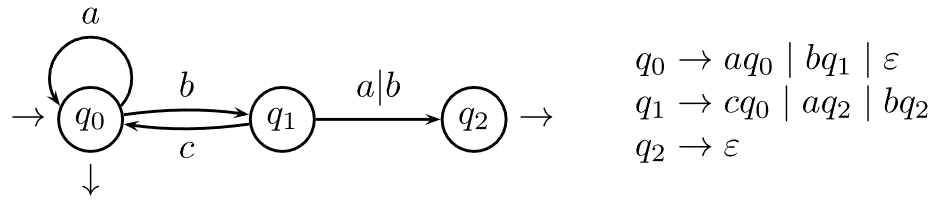
\includegraphics[width=0.9\linewidth]{images/autgram.png}
        \end{figure}
    \end{example}
    The conversion from automaton to grammar has been straightforward, but to make the reverse transformation from grammar to automaton, we need to 
    modify the machine definition by permitting nondeterministic behavior.
        
    \section{Nondeterministic automata}
    A right-linear grammar may contain two alternative rules starting with the same character. In this case, converting the rules to machine transitions, two arrows with 
    identical label would exit from the same state $A$ and enter two distinct states $B$ and $C$. This means that in state $A$, reading the character, the machine can 
    choose which one of the next states to enter: its behavior is not deterministic. A machine move that does not read an input character is termed spontaneous or an epsilon 
    move. Spontaneous moves too cause the machine to be nondeterministic. 

    \subsection{Motivation of non-determinism}
    The main advantages of this are: 
    \begin{itemize}
        \item Concision: defining a language with a nondeterministic machine often results in a more read-able and compact definition. 
        \item Left right interchange and language reflection: it is useful when a deterministic machine is used to recognize the reflection. 
        \item Converting regular expressions to automaton. 
    \end{itemize}

    \subsection{Nondeterministic recognizers}
    \begin{definition}
        A \emph{non-deterministic finite automaton} $N$, without spontaneous moves, is defined by: 
        \begin{itemize}
            \item The state set $Q$. 
            \item The terminal alphabet $\Sigma$. 
            \item Two subsets of $Q$: the set $I$ of the initial states and the set $F$ of final states.
            \item The transition relation $\delta$, a subset of the Cartesian product $Q\times\Sigma\times Q$.     
        \end{itemize}
\end{definition} 
    As before, a computation is a series of transitions such that the origin of each one coincides with the destination of the preceding one. The computation
    origin is $q_0$, the termination is $q_n$, and the length is the number $n$ of transitions or moves. A computation of length 1 is just a transition.
    A string $x$ is recognized or accepted by the automaton, if it is the label of a computation originating in some initial state, terminating in some final state, 
    and having label $x$. The language $L(N)$ recognized by automaton $N$ is the set of accepted strings. The moves of a nondeterministic automaton can still be 
    considered as a finite function, but one computing sets of values. For a machine $N=(Q,\Sigma,\delta,I,F)$, devoid of spontaneous moves, the functionality of the 
    state-transition function $\delta$ is the following: 
    \[\delta:Q\times\left(\Sigma\cup\{\varepsilon\}\right)\rightarrow \mathcal{P}(Q)\]
    where symbol $\mathcal{P}(Q)$ indicates the power set of set $Q$. 

    \subsection{Automata with spontaneous moves}
    Another kind of nondeterministic behavior occurs when an automaton changes state without reading a character, thus performing a spontaneous move. In this case 
    the number of steps of the computation can exceed the length of the input string, because of the presence of $\varepsilon$-arcs. As a consequence, the recognition 
    algorithm no longer works in real time. Yet time complexity remains linear, because it is possible to assume that there are no cycles of spontaneous moves in any 
    computation. The family of languages recognized by such nondeterministic automata is also called finite-state.

    The official definition of nondeterministic machine allows two or more initial states, but it is easy to construct an equivalent machine with only one: add to the
    machine anewstateq0, which will be the only initial state, and the $\varepsilon$-arcs going from it to the former initial states of the automaton.

    \subsection{Correspondence between automata and grammars}
    Consider a right-linear grammar $G=(V,\Sigma,P,S)$ and a nondeterministic automaton $N=(Q,\Sigma,\delta,q_0,F)$, which we may assume from the preceding discussion to 
    have a single initial state. First assume the grammar rules are strictly unilinear. The states $Q$ of the automaton match the non-terminals $V$ of the grammar. The 
    initial state corresponds to the axiom. Notice that the pair of alternatives $p\rightarrow aq|ar$ correspond to two nondeterministic moves. A copy rule matches a 
    spontaneous move. A final state  matches a non-terminal having an empty rule.
    \begin{figure}[H]
        \centering
        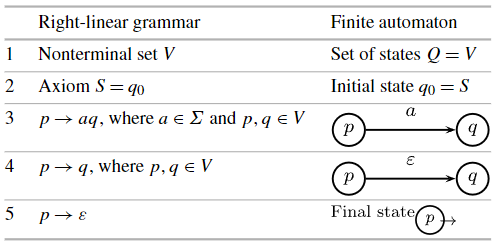
\includegraphics[width=0.75\linewidth]{images/correspondence.png}
        \caption{Correspondence between automaton and grammar}
    \end{figure}

    \subsection{Ambiguity of automata}
    \begin{definition}
        An automaton is \emph{ambiguous} if it accepts a string with two different computations.
    \end{definition}
    Clearly it follows from the definition that a deterministic automaton is never ambiguous. We also have that an automaton is ambiguous if, and only if, the right-linear 
    equivalent grammar is ambiguous. 

    REG families can be defined also using left-linear grammars. By interchanging left with right, it is simple to discover the mapping between such grammars and automata.

    \section{From automaton to regular expression: the BMC method}
    Suppose for simplicity the initial state $i$ is unique, and no arc enters in it; similarly the final state $t$ is unique and without outgoing arcs. Otherwise, just add
    a new initial state $i$ connected by spontaneous moves to the ex-initial states; similarly introduce a new unique final state $t$. Every state other than $i$ and $t$ is 
    called internal. We construct an equivalent automaton, termed generalized,  which is more flexible as it allows arc labels to be not just terminal characters, but also 
    regular languages. The idea is to eliminate one by one the internal states, while compensating by introducing new arcs labeled with regular expression, until only the initial and final 
    states are left. Then the label of arc $i \rightarrow t$ is the regular expression of the language.
    \begin{example}
        The BMC method applied to a simple automaton: 
        \begin{figure}[H]
            \centering
            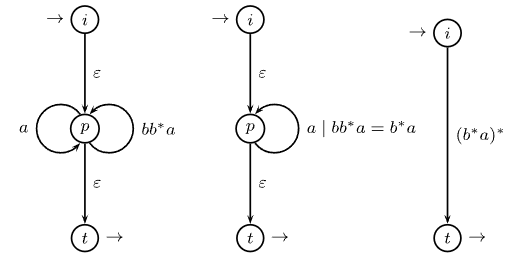
\includegraphics[width=0.6\linewidth]{images/brzozowski.png}
        \end{figure}
    \end{example}

    \section{Elimination of non-determinism}
    Every non-deterministic finite automaton can always be transformed into an equivalent deterministic one. Consequently, every right linear grammar always admits an 
    equivalent non-ambiguous right linear one. Thus,  every ambiguous regular expression can always be transformed into a non-ambiguous one. The algorithm to transform a 
    non-deterministic automaton into a deterministic one is structured in two phases: 
    \begin{enumerate}
        \item Elimination of the spontaneous moves. As such moves correspond to copy rules, it suffices to apply the algorithm for removing the copy rules. 
        \item Replacement of the non-deterministic multiple transitions by changing the automaton state set. This is the well known subset construction. 
    \end{enumerate}
    \begin{example}
        Given the following automaton: 
        \begin{figure}[H]
            \centering
            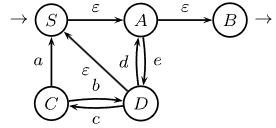
\includegraphics[width=0.5\linewidth]{images/oaut.png}
        \end{figure}
        After applying the algorithm we have: 
        \begin{figure}[H]
            \centering
            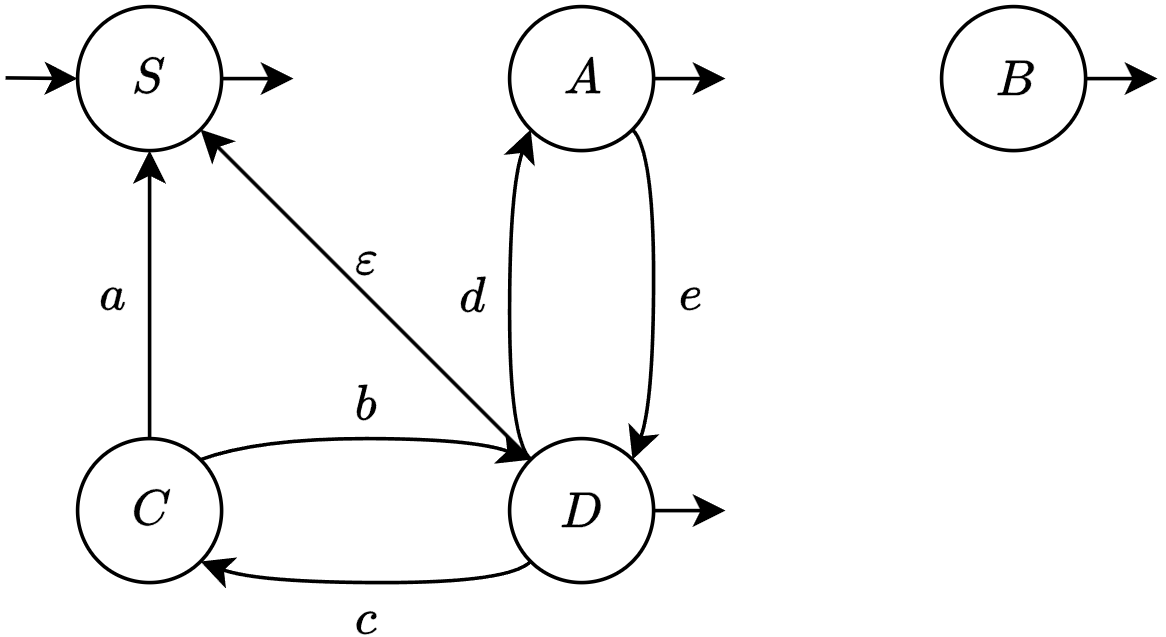
\includegraphics[width=0.5\linewidth]{images/faut.png}
        \end{figure}
    \end{example}

    \section{From a regular expression to a finite state automaton}
    There are a few algorithms to transform a regular expression into an automaton, which differ as for automaton characteristic. 
    
    \subsection{Thompson structural method}
    Wit the Thompson structural method, given a regular expression, we analyze it into simple parts, we produce corresponding component automata, and we interconnect them 
    to obtain the complete recognizer. In  this  construction each  component machine is  assumed to  have  exactly one initial state without incoming arcs and one final 
    state without outgoing arcs. 
    \begin{figure}[H]
        \centering
        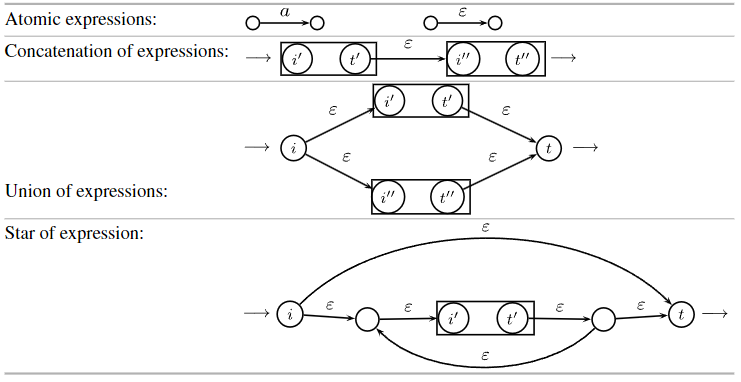
\includegraphics[width=1\linewidth]{images/thompson.png}
        \caption{Sub-expression to automaton}
    \end{figure}
    The validity of Thompson's method comes from it being an operational reformulation of the closure properties of regular languages under concatenation, union, and star.
    In general the outcome of the Thompson method is a non-deterministic automaton with spontaneous moves. There are various optimizations of the Thompson method that avoid 
    creating redundant states. 

    \subsection{Glushkov-McNaughton-Yamada algorithm}
    The GMY algorithm constructs the automaton equivalent to a given regular expression, with states that are in a one-to-one correspondence with the generators that occur
    in the regular expression. 

    \begin{definition}
        Given a language $L$ over the alphabet $\Sigma$ we can define: 
        \begin{itemize}
            \item The set of initials: $Ini(L)=\{a \in \Sigma | a\Sigma^{*}\cap L \neq \varnothing\}$. 
            \item The set of finals: $Fin(L)=\{a \in \Sigma | \Sigma^{*}a\cap L \neq \varnothing\}$.
            \item The set of digrams: $Dig(L)=\{x \in \Sigma^{2} | \Sigma^{*}x\Sigma^{*} \cap L \neq \varnothing\}$.
            \item The set of forbidden digrams: $\overline{Dig(L)}=\Sigma^{2}-Dig(L)$
        \end{itemize}
        The language $L$ is called \emph{local} or \emph{locally testable}, if and only if it satisfies the following identity: 
        \[L-\{\varepsilon\}=\{x|Ini(x)\in Ini(L) \land Fin(x)\in Fin(L)\land Dig(x)\subseteq Dig(L)\}\]
    \end{definition}
    To design the recognizer of a local language we scan the input string from left to right and check whether: the initial character belongs to the set $Ini$, every 
    digram belongs to the set $Dig$, and the final character belongs to the set $Fin$. The string is accepted if, and only if, all the above checks succeed. 

    We can implement the above recognizer by resorting to a sliding window with a width of two characters, which is shifted over the input string from left to right.
    At each shift step the window contents are checked, and if the window reaches the end of the string and all the checks succeed, then the string is accepted, otherwise
    it is rejected. This sliding window algorithm is simple to implement by means of a non-deterministic automaton. 
    \begin{definition}
        A regular expression is said to be \emph{linear} if there is not any repeated generator. 
    \end{definition}
    The idea of the GMY algorithm, based on the linear regular expressions is the following: 
    \begin{enumerate}
        \item Denumerate the regular expression e and obtain the linear regular expression $e_{\#}$. 
        \item Compute the three characteristic local sets $Ini$, $Fin$ and $Dig$ of $e_{\#}$.
        \item Design the recognizer of the local language generated by $e_{\#}$.
        \item Cancel the indexing and thus obtain the recognizer of $e$.
    \end{enumerate}
    
    \subsection{Berry-Sethi method}
    In order to obtain the deterministic recognizer, we can just apply the subset construction to the non-deterministic recognizer built by the GMY algorithm. However, there 
    is a more direct algorithm called Berry-Sethi. The idea at the base of this algorithm is the following: 
    \begin{enumerate}
        \item From the original regular expression $e$ over alphabet $\Sigma$ derive the linear expression $e^{'}\dashv$, where $e^{'}$ is the numbered version of $e$ 
            and $\dashv$ is a string terminator symbol, with $\dashv \notin \Sigma$.
        \item Build the local automaton recognizing the local language $L(e^{'}\dashv)$: this automaton includes the initial state $q_0$, one non-initial and non-final
            state for each element of $\Sigma_N$, and a unique final state $\vdash$.
        \item Label each state of the automaton with the set of the symbols on its outgoing edges. The initial state $q_0$ is labeled with $Ini(e^{'}\dashv)$, the final 
            state $\dashv$ is labeled with the empty set $\varnothing$. For each non-initial and non-final states $c$, $c \in \Sigma_N$, the set labeling that state is 
            called the set of followers of symbol $c$, $Fol(c)$,in the expression $e^{'}\dashv$; it is derived directly from the local set of digrams as follows:
            $Fol(a_i)=\{b_j|a_ib_j \in Dig(e^{'}\dashv)\}$. $Fol$ is equivalent to the $Dig$ local set and, together with the other two local sets $Ini$ and $Fin$, 
            characterizes a local language.
        \item Merge any existing states of the automaton that are labeled by the same set. The obtained automaton is equivalent to the previous one: since the recognized 
            language is local, states marked with equal sets of followers are indistinguishable
        \item Remove the numbering from the symbols that label the transitions of the automaton: the resulting automaton, which may be nondeterministic, accepts by 
            construction the language $L(e^{'}\dashv)$.
        \item Derive a deterministic, equivalent automaton by applying the construction of Accessible Subsets; label the sets resulting from the union of several states of 
            the previous nondeterministic automaton with the union of the sets labeling the merged states. The resulting deterministic automaton recognizes $L(e^{'}\dashv)$.
        \item Remove from the automaton the final state (labeled by $\varnothing$) and all arcs entering it; define as final states of the resulting automaton those labeled 
            by a set that includes the $\dashv$ symbol; the resulting automaton is deterministic and recognizes $L(e)$.
    \end{enumerate}
    \begin{algorithm}[H]
        \caption{Berry-Sethi algorithm}
            \begin{algorithmic}[1]
                \State $q_0 \leftarrow Ini(e_{\#} \dashv)$
                \State $Q \leftarrow \{q_0\}$
                \State $\delta \leftarrow \varnothing$
                \While {$\exists q \in Q$ such that $q$ is unmarked}
                    \State mark state $q$ as visited
                    \For {each character $c \in \Sigma$}
                        \State $q^{'} \leftarrow \bigcup_{\forall c_{\#} \in \Sigma_{c_{\#}}}Fol(c_{\#})$
                        \If {$q^{'} \neq \varnothing$}
                            \If {$q^{'} \notin Q$}
                                \State set $q^{'}$ as a new unmarked state
                                \State $Q \leftarrow Q \cup \{q^{'}\}$
                            \EndIf
                            \State $\delta \leftarrow Q \cup \{q^{'}\}$
                        \EndIf
                    \EndFor
                \EndWhile
            \end{algorithmic}
    \end{algorithm}
    \begin{example}
        Given the language $L=(a|bb)^{*}(ac)^{+}$ apply the BS algorithm. First we enumerate the string: 
        \[e_{\#}=(a_1|b_2b_3)^{*}(a_4c_5)^{+} \dashv\]
        And with the table we obtain:
        \begin{figure}[H]
            \centering
            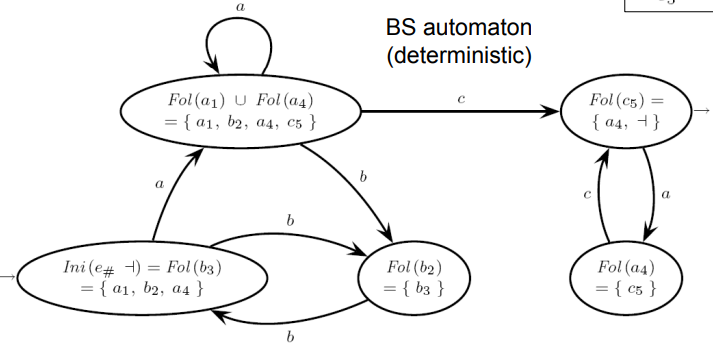
\includegraphics[width=0.8\linewidth]{images/BS.png}
        \end{figure}
    \end{example}
    Another use of algorithm BS is as an alternative to the power set construction, for converting a nondeterministic machine $N$ into a deterministic one $M$. The steps are: 
    \begin{enumerate}
        \item Distinctly number the labels of non-$\varepsilon$ arcs of $N$, obtaining automaton $N^{'}$.
        \item Compute the local sets $Ini$, $Fin$, and $Fol$ for the language $L(N^{'})$. These can be easily derived from the transition graph, possibly exploiting the 
            identity $\varepsilon a=a\varepsilon=a$.
        \item Applying the BS construction to the sets $Ini$, $Fin$, and $Fol$, produce the deterministic automaton $M$.
    \end{enumerate}

    \section{Regular expression: complement and intersection}
    Regular expressions may also contain the operators of complement, intersection and set difference, which are very useful to make the regexp more concise. 
    Let $L$ and $L^{'}$ be regular languages. The complement $\lnot L$ and the intersection$L \cap L^{'}$ are regular languages. The deterministic recognizer $\overline{M}$ 
    of the complement language requires to complete the automaton $M$ by adding the error state p and the missing moves: 
    \begin{itemize}
        \item Create the error state $p$, not in $Q$, so the states of $\overline{M}$ are $Q \cup \{ p \}$
        \item The transition function $\delta$ is: 
            \begin{itemize}
                \item $\delta(q,a)=\delta(q,a)$, where $\delta(q,a) \in Q$. 
                \item $\delta(q,a)=p$, where $\delta(q,a)$ is not defined;
                \item $\delta(p,a)=p$, for every character $a \in \Sigma$;
            \end{itemize}
        \item Swap the non-final and final states. 
    \end{itemize}
    \begin{example}
        Find the complement of the given automaton: 
        \begin{figure}[H]
            \centering
            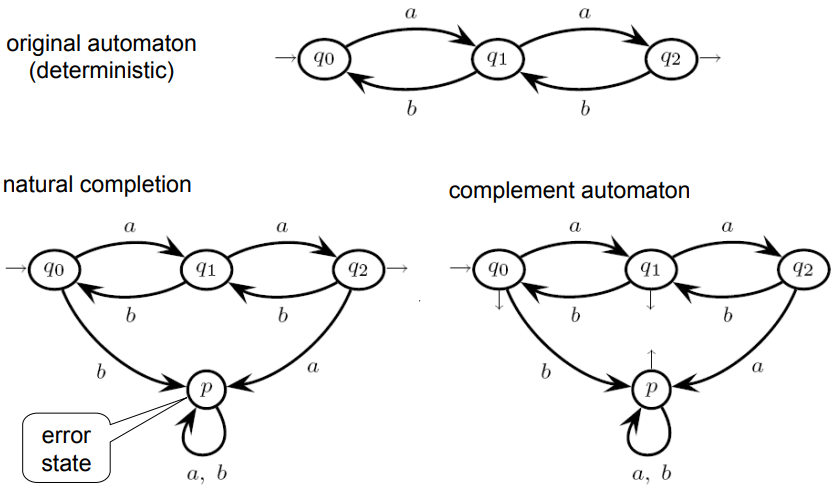
\includegraphics[width=0.8\linewidth]{images/complement.png}
        \end{figure}
    \end{example}
    For the complement construction to work correctly, the original automaton must be deterministic, otherwise the original and complement languages may be not disjoint,
    which fact would be in violation of the complement definition. The complement automaton may contain useless states and may not be in the minimal form either; it should 
    be reduced and minimized, if necessary. 
    \subsection{Product of automata}
    A very common construction of formal languages, where a single automaton simulates the computation of two automata that work in parallel on the same input string. 
    It is very useful to construct the intersection automaton. To obtain the intersection automaton we can resort to the De Morgan theorem. The Cartesian product can 
    also be obtained by a more direct construction. The intersection of the two languages is recognized directly by the Cartesian product of their automata. 
    Suppose both automata do not contain any spontaneous moves. The state set of the product machine is the Cartesian product of the state sets
    of the two automata. Each product state is a pair $\left\langle q^{'},q^{''} \right\rangle $, where the left (right) member is a state of the first (second) machine. 
    The move is: 
    \[\left\langle q^{'},q^{''} \right\rangle \rightarrow^a \left\langle r^{'},r^{''} \right\rangle \textnormal{ if and only if } q^{'} \rightarrow r^{'} \textnormal{ and } q^{''} \rightarrow r^{''}\]
    The product machine has a move if, and only if, the projection of such a move onto the left (right) component is a move of the first (second) automaton. The initial 
    and final state sets are the Cartesian products of the initial and final state sets of the two automata, respectively. The product construction is equivalent to simulating both 
    machines in parallel.
    \begin{example}
        The intersection can be found as follows: 
        \begin{figure}[H]
            \centering
            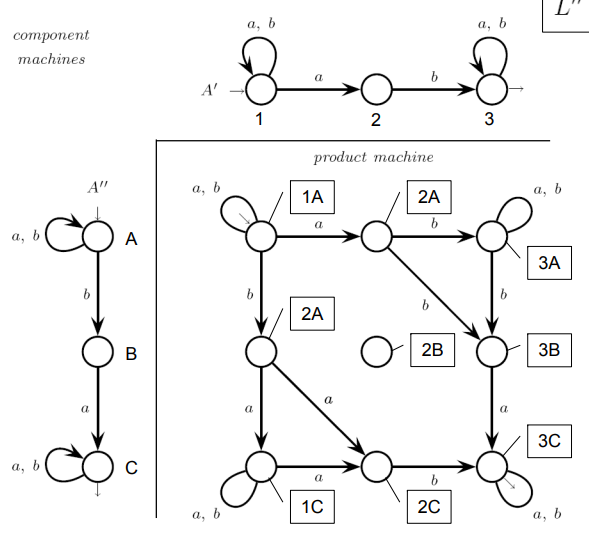
\includegraphics[width=0.52\linewidth]{images/intersection.png}
        \end{figure}
    \end{example}
\end{document}